\documentclass[10pt]{article}

\pagestyle{empty}

\setlength{\textheight}{250mm}
\setlength{\textwidth}{180mm}
\setlength{\oddsidemargin}{-8mm}
\setlength{\topmargin}{-1.5cm}

\usepackage{amsmath}
\usepackage{amsthm}
\usepackage{psfrag}
\usepackage{graphicx}
\usepackage{bm}
\usepackage{mathrsfs}
\usepackage{icomma} % pacchetto per limitare lo spazio standard posto dopo la virgola in caso che la virgola sia tra cifre
\usepackage{amsfonts} % amplia i caratteri matematici disponibili
\usepackage{amssymb}
%\usepackage{wrapfig}
\usepackage{empheq}

\usepackage{epstopdf}
\usepackage[utf8x]{inputenc}
\usepackage{ifthen}

\usepackage[italian]{babel}
%\usepackage[latin1]{inputenc}

\usepackage{pgfplots}
\pgfplotsset{compat=1.9}

%\input{def}

%\newcommand{\kg}{\textrm{kg}}
%\newcommand{\K}{\textrm{K}}
%\newcommand{\m} {\textrm{m}}
%\newcommand{\dm}{\textrm{dm}}
%\newcommand{\cm}{\textrm{cm}}
%\newcommand{\mm}{\textrm{mm}}
%\newcommand{\s} {\textrm{s}}
%\newcommand{\N} {\textrm{N}}
%\renewcommand{\Pa}{\textrm{Pa}}

\def \flagSect{0} % 1    : numerazione
		  % else : niente
%\newcommand{\taitol}[1]  % stile titolo
%{
%%{\textit{#1}}
%{#1}
%}
\def \soluzione{Soluzione}
\def \partePrima{Concetti. }
\def \parteSeconda{Svolgimento. }
%\def \parteTerza{}
\newcommand{\sol}{\subsubsection*{\soluzione}}
\newcommand{\partone}{\ \ \ \ \ \textbf{\partePrima}}
\newcommand{\parttwo}{\vspace{0.2cm}\textbf{\parteSeconda}}

\ifnum\flagSect=1
\newtheorem{esercizio}{Esercizio}%[section]
\else
\newtheorem*{esercizio}{Esercizio}
\fi

\newtheorem*{teorema}{Teorema}
\newtheorem*{lemma}{Lemma}

% ###########################################################
%\def \flagSect{0} % 1    : numerazione
		  % else : niente
%\newcommand{\taitol}[1]  % stile titolo
%{
%%{\textit{#1}}
%{#1}
%}
\def \soluzione{Soluzione}
\def \partePrima{Concetti. }
\def \parteSeconda{Svolgimento. }
%\def \parteTerza{}
\newcommand{\sol}{\subsubsection*{\soluzione}}
\newcommand{\partone}{\ \ \ \ \ \textbf{\partePrima}}
\newcommand{\parttwo}{\vspace{0.2cm}\textbf{\parteSeconda}}

\ifnum\flagSect=1
\newtheorem{esercizio}{Esercizio}%[section]
\else
\newtheorem*{esercizio}{Esercizio}
\fi

\newtheorem*{teorema}{Teorema}
\newtheorem*{lemma}{Lemma}

% ###########################################################
%\def \flagSect{0} % 1    : numerazione
		  % else : niente
%\newcommand{\taitol}[1]  % stile titolo
%{
%%{\textit{#1}}
%{#1}
%}
\def \soluzione{Soluzione}
\def \partePrima{Concetti. }
\def \parteSeconda{Svolgimento. }
%\def \parteTerza{}
\newcommand{\sol}{\subsubsection*{\soluzione}}
\newcommand{\partone}{\ \ \ \ \ \textbf{\partePrima}}
\newcommand{\parttwo}{\vspace{0.2cm}\textbf{\parteSeconda}}

\ifnum\flagSect=1
\newtheorem{esercizio}{Esercizio}%[section]
\else
\newtheorem*{esercizio}{Esercizio}
\fi

\newtheorem*{teorema}{Teorema}
\newtheorem*{lemma}{Lemma}

% ###########################################################
%\input{logicNumb}
%\newcommand{\sectionIf}[2]
%{
%   \ifthenelse{\equal{#1}{1}}
%              {\subsection{#2}}{\subsection*{#2}}
%}
% ###########################################################

%\newcommand{\sectionIf}[2]
%{
%   \ifthenelse{\equal{#1}{1}}
%              {\subsection{#2}}{\subsection*{#2}}
%}
% ###########################################################

%\newcommand{\sectionIf}[2]
%{
%   \ifthenelse{\equal{#1}{1}}
%              {\subsection{#2}}{\subsection*{#2}}
%}
% ###########################################################


\begin{document}

\begin{center}
\textbf{Esercizi per il corso di Fluidodinamica} 
\medskip
\end{center}

\noindent
\begin{tabular}{c}
\begin{minipage}[b]{0.95\textwidth}
\begin{exerciseS}[Potenziale cinetico e funzione di corrente]
Si consideri la corrente a potenziale piana e stazionaria descritta in un sistema
di riferimento Cartesiano $(x,y)$ dalla funzione potenziale cinetico $\phi(x,y)$:
$$
 \phi(x,y) = 5(x^2-y^2) + 2x-4y.
$$
Si richiede di:
\begin{itemize}
 \item derivare l'espressione analitica delle componenti in $x$ e in $y$ del campo di velocit\`{a};
 \item verificare che la corrente sia incomprimibile e irrotazionale;
 \item derivare l'espressione analitica della funzione di corrente $\psi(x,y)$;
 \item calcolare la portata volumetrica per unit\`{a} di apertura $q$ che scorre attraverso il 
       segmento congiungente l'origine del piano con il punto di coordinate $(1,1)$;
\end{itemize}
\vspace{0.2cm}
($u_x=10x+2$, $u_y=-10y-4$, $\psi(x,y)=10xy+2y+4x + const.$, $q=16$)
\end{exerciseS}
\end{minipage}
\end{tabular}


\sol

\partone
  Legame tra potenziale e velocità. Funzione di corrente per problemi 2D incomprimibili.
\begin{equation}
  \bm{u} = \bm{\nabla} \phi \quad
  \begin{cases}
  \begin{aligned}
   & u_x  =  \frac{\partial \phi}{\partial x}  = \frac{\partial \psi}{\partial y} \\
   & u_y  =  \frac{\partial \phi}{\partial y}  = - \frac{\partial \psi}{\partial x}
  \end{aligned}
  \end{cases}
\end{equation}

\parttwo

\begin{itemize}

\item Calcolo delle componenti della velocità.
\begin{equation}
  \begin{cases}
    u_x = \frac{\partial \phi}{\partial x} = 10 x + 2 \\
    u_y = \frac{\partial \phi}{\partial y} = -10 y - 4
  \end{cases}
\end{equation}

\item Verificare che la corrente sia incomprimibile e irrotazionale.
  \begin{itemize}
    \item Irrotazionalità ($\nabla \times \bm{u} = 0$). Verifica tramite l'identità vettoriale $\nabla \times \nabla \phi = 0$, oppure con il calcolo diretto.
    \begin{equation}
    \begin{aligned}
      & \nabla \times \bm{u} = \nabla \times (\nabla \phi) = 0 \\
      & \nabla \times \bm{u} = \nabla \times ( (10x+2)\hat{\bm{x}} + (-10y-4)\hat{\bm{y}} ) = 
      \displaystyle \left(\frac{\partial u_y}{\partial x} - \frac{\partial u_x}{\partial y} \right)\hat{\bm{z}} = 0
    \end{aligned}
    \end{equation}
        
    \item Incomprimibilità ($\nabla \cdot \bm{u} = 0$). Dal calcolo diretto $\partial^2 \phi /\partial x^2 + \partial^2 \phi /\partial y^2=10-10=0$.
    
  \end{itemize}
  
  \item La corrente è incomprimibile, quindi si può definire la funzione di corrente. Usando la definizione della funzione di corrente, integrando, si ottiene:
  
  \begin{equation}
  \begin{aligned}
    &\frac{\partial \psi}{\partial y} = u_x   &\quad \Rightarrow \quad \psi = 10xy+2y+f(x)\\
    &\frac{\partial \psi}{\partial x} = -u_y  &\quad \Rightarrow \quad \psi = 10xy+4x+g(y)
  \end{aligned}
  \end{equation}
  
  \begin{equation}
    \psi = 10 xy + 2y + 4x + c
  \end{equation}
  
  \item Calcolo della portata.
  \begin{equation}
    Q = \int_{\gamma} \bm{u} \cdot \hat{\bm{n}} = \int_{\gamma} (u_x n_x + u_y n_y) = 
    \int_{\gamma} (u_x t_y - u_y t_x) = 
    \int_{\gamma} \displaystyle\left(\frac{\partial \psi}{\partial x} t_x + \frac{\partial \psi}{\partial y} t_y\right) = 
    \psi(1,1) - \psi(0,0) = 16
  \end{equation}

\end{itemize}



\newpage
\clearpage
\noindent
\begin{tabular}{c}
\begin{minipage}[b]{0.95\textwidth}
\begin{exerciseS}[Corrente attorno al cilindro]
Una corrente piana con velocit\`{a} asintotica $U_\infty=10\ m/s$ investe un profilo circolare
di raggio $a=0.1\ m$. Determinare il valore di circolazione $\Gamma$ affinch\'{e} nel 
punto sulla superficie del cilindro posto a $\theta=\pi/3$ la velocit\`{a} aumenti fino al valore 
$2U_\infty$ in modulo.

($\Gamma = -1.68\ m^2 / s$, 23.45$\ m^2 / s$)
\end{exerciseS}
\end{minipage}
\end{tabular}


\sol

\partone
  Flusso non viscoso 2D, incomprimibile e irrotazionale attorno al cilindro. Circolazione

\parttwo
 Una volta scritte (come si ricavano?) le componenti della velocità nel campo di moto, si
impongono le condizioni richieste dal problema per determinare il valore di circolazione necessario.

\begin{equation}
\begin{cases}
  u_r (r,\theta) = U_\infty \displaystyle \left(1 - \frac{a^2}{r^2}\right)\cos{\theta} \\
  u_\theta (r,\theta) = - U_\infty \displaystyle \left(1 + \frac{a^2}{r^2}\right)\sin{\theta} + \frac{\Gamma}{2\pi r}
\end{cases}
\end{equation}

\vspace{0.2cm}
Si impongono ora le condizioni del problema. Sulla superficie del cilindro la componente radiale è nulla (condizioni al contorno). Quindi:

\begin{equation}
  |\bm{u}(a,\theta)| = |u_\theta(a,\theta)| = \Big| - 2 U_\infty \sin{\theta} + \frac{\Gamma}{2 \pi a} \Big|
\end{equation}

E quindi
\vspace{0.2cm}
\begin{equation}
\begin{aligned}
  2 U_\infty & = \Big| - 2 U_\infty \sin{\frac{\pi}{3}} + \frac{\Gamma}{2 \pi a} \Big| \\
  \pm 2 U_\infty & = - 2 U_\infty \frac{\sqrt{3}}{2} + \frac{\Gamma}{2 \pi a} \\
  \\
  \Rightarrow \Gamma  & = 2 \pi a U_\infty (\sqrt{3} \pm 2)
\end{aligned}
\end{equation}

\begin{equation}
  \Rightarrow \Gamma = 
  \begin{cases}
    -1.684 \ m^2/s \\
    23,449 \ m^2/s
  \end{cases}
\end{equation}


\newpage
\clearpage
\noindent
\begin{tabular}{c}
\begin{minipage}[b]{0.95\textwidth}
\begin{exerciseS}[Corrente attorno al cilindro]
Una corrente piana con velocit\`{a} asintotica orizzontale (parallela all'asse x) $U_\infty=1$ viene perturbata introducendo 
nell'origine del piano un vortice in modo tale da accelerare la corrente nel semipiano superiore e rallentarla 
in quello inferiore per valori positivi di $\Gamma$. Determinare la circolazione necessaria ad ottenere una differenza di componente x della velocit\`{a} pari a 1 
tra i due punti di coordinate (polari) $R=1$ e $\theta=\pm\pi/2$. 
($\Gamma = -\pi$)
\end{exerciseS}
\end{minipage}
\end{tabular}

\sol

\partone
 Flusso non viscoso 2D, incomprimibile e irrotazionale. Circolazione. Corrente indisturbata. Vortice. Sovrapposizione delle cause e degli effetti.

\parttwo
 Una volta scritte (come si ricavano?) le componenti della velocità nel campo di moto, si
impongono le condizioni richieste dal problema per determinare il valore di circolazione necessario.

\begin{equation}
\begin{cases}
  u_r (r,\theta) = U_\infty \cos{\theta} \\
  u_\theta (r,\theta) = - U_\infty \sin{\theta} + \frac{\Gamma}{2\pi r}
\end{cases}
\end{equation}

\vspace{0.2cm}
Si impongono ora le condizioni del problema. Per $\theta_1 = \pi/2$ e $\theta_2 = -\pi/2$, la componente radiale è nulla.

\begin{equation}
  \begin{cases}
    u_{\theta}(R,\theta_1) = -U_\infty + \frac{\Gamma}{2\pi R} \\
    u_{\theta}(R,\theta_2) = U_\infty + \frac{\Gamma}{2\pi R}
  \end{cases}
\end{equation}

Si vuole determinare la differenza delle componenti in direzione x $u_x(R,\theta_1) - u_x(R,\theta_2)$; questa è uguale a $-(u_\theta(R,\theta_1) + u_\theta(R,\theta_2))$. Quindi, per $R=1$:

\begin{equation}
  -\frac{\Gamma}{\pi} = 1 \quad \Rightarrow \quad \Gamma = -\pi
\end{equation}


\newpage
\clearpage
\noindent
\begin{tabular}{c}
\begin{minipage}[b]{0.5\textwidth}
 \begin{exerciseS}[Semicilindro. Risultante delle forze]
  Si consideri la copertura rigida di un campo da calcio avente sezione semicircolare di
  raggio $\bar{R}=50\ m$ rappresentata schematicamente in figura. Sulla struttura 
  soffia un vento uniforme ($\rho=1.225\,kg/m^3$, $P_\infty=101325\ Pa$) in direzione 
  orizzontale con velocit\`{a} $U_\infty=15\,km/h$. Assumendo di poter approssimare la corrente esterna 
  come stazionaria, bidimensionale e a potenziale, si richiede di determinare:
  \begin{itemize}
   \item[1.1)] la distribuzione della pressione esterna sulla sezione della struttura;
   \item[1.2)] la risultante per unit\`{a} di apertura delle forze agenti sulla struttura, 
               ipotizzando che la pressione interna $P_i$ sia pari a $P_\infty$.
  \end{itemize}
  \vspace{2mm}
($P(\theta) = P_\infty+\frac{1}{2}\rho U_\infty^2(1-4\sin^2\!\theta)$, $\bm{F} = 425.35\mathbf{\hat{\bm{y}}}\ N/m$)
  \end{exerciseS}
\end{minipage}
\hspace{3mm}
\begin{minipage}[b]{0.35\textwidth}
   \begin{center}
   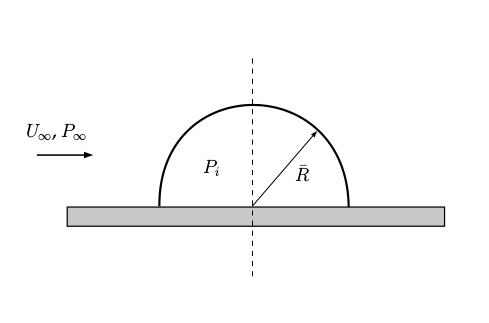
\includegraphics[width=1.50\textwidth]{./fig/Cyl.png}
   \end{center}
\end{minipage}
\end{tabular}


\sol

\partone
 Flusso non viscoso 2D, incomprimibile e irrotazionale attorno al cilindro. Circolazione.

\parttwo
 Una volta scritte (come si ricavano?) le componenti della velocità nel campo di moto, tramite il teorema di Bernoulli (nel caso incomprimibile, stazionario, inviscido, irrotazionale,...) si calcola la pressione agente sulla superficie del cilindro. Integrando gli sforzi di pressione (interna ed esterna al cilindro) sul contorno, si ottiene la risultante.

\begin{itemize}

\item Campo di moto nel dominio esterno alla metà cilindro ($(r,\theta) \in [0,\infty)\times[0,\pi])$.

\begin{equation}
\begin{cases}
  u_r (r,\theta) = U_\infty \displaystyle \left(1 - \frac{a^2}{r^2}\right)\cos{\theta} \\
  u_\theta (r,\theta) = - U_\infty \displaystyle \left(1 + \frac{a^2}{r^2}\right)\sin{\theta}
\end{cases}
\end{equation}

\item Grazie al teorema di Bernoulli (ipotesi...) si ottiene la pressione esterna sulla superficie della metà di cilindro. Sulla superficie del cilindro la componente radiale è nulla, quindi il modulo della velocità coincide con il valore assoluto della componente radiale.
\begin{equation}
\begin{aligned}
  P(\theta) & = P_\infty + \frac{1}{2}\rho U_\infty^2 - \frac{1}{2}\rho u_\theta(a,\theta)^2 = \\
            & = P_\infty + \frac{1}{2}\rho U_\infty^2 - \frac{1}{2}\rho (2 U_\infty \sin{\theta})^2 = \\
            & = P_\infty + \frac{1}{2}\rho U_\infty^2 (1 - 4 \sin^2{\theta})
\end{aligned}
\end{equation}

\item Integrale sulla superficie (interna ed esterna) degli sforzi di pressione per ottenere la risultante. Con $\hat{\bm{b}}$ si indica la normale diretta verso il centro del cilindro.

\begin{equation}
\begin{aligned}
  \bm{F} & = \int_{0}^{\pi} (P(\theta)-P_\infty) \hat{\bm{b}} a d\theta = \\
      & = \int_{0}^{\pi} (\frac{1}{2}\rho U_\infty^2 (1 - 4 \sin^2{\theta}) (-\cos{\theta}\hat{\bm{x}} - \sin{\theta}\hat{\bm{y}}) a d\theta = \\
\end{aligned}
\end{equation}

\vspace{0.2cm}
Usando i risultati (integrare!!)
\begin{equation}
\begin{aligned}
 & \int_{0}^{\pi} \sin{\theta} d\theta  = 2 \\
 & \int_{0}^{\pi} \cos{\theta} d\theta  = 0 \\
 & \int_{0}^{\pi} \sin^3{\theta} d\theta  = \frac{4}{3} \\
 & \int_{0}^{\pi} \cos{\theta}\sin^2{\theta} d\theta  = 0 
\end{aligned}
\end{equation}

si ottiene:
\begin{equation}
\begin{aligned}
  \bm{F} & = \int_{0}^{\pi} (P(\theta)-P_\infty) \hat{\bm{b}} a d\theta = \\
      & = - \frac{1}{2}\rho a U_\infty^2 \int_{0}^{\pi}  (1 - 4 \sin^2{\theta}) \sin{\theta}\hat{\bm{y}} d\theta = \\
      & = - \frac{1}{2}\rho a U_\infty^2 \displaystyle\left( 2 - \frac{16}{3}\right)\hat{\bm{y}} \\ \\
  \bm{F} & = \frac{5}{3}\rho a U_\infty^2 \hat{\bm{y}} \quad \Rightarrow \quad \bm{F} = 425.35 \hat{\bm{y}} N/m
\end{aligned}
\end{equation}


\end{itemize}

\newpage
\clearpage
\subsection{Condizione necessaria di incipiente separazione}
Un punto di incipiente separazione viene identificato dall'anullarsi
 della derivata in direzione perpendicolare a parete della componente
 di velocità parallela ad essa, con derivata seconda positiva.
Si consideri il problema bidimensionale su una superficie piana: viene
 scelto di usare un sistema di riferimento cartesiano con l'asse $x$
 parallelo alla parete e diretto nel verso della corrente asintotica
 $\bm{U} = U \bm{x}$, l'asse $y$ uscente dalla parete.
La componente $x$ dell'equazione della quantità di moto è
 \begin{equation}
  u \dfrac{\partial u}{\partial x} +
  v \dfrac{\partial u}{\partial y} -
  \dfrac{1}{Re}\left[ \dfrac{\partial^2 u}{\partial x^2} +
                      \dfrac{\partial^2 u}{\partial y^2} \right] +
  \dfrac{\partial P}{\partial x} = 0
 \end{equation}
A parete i termini non lineari sono nulli poichè la velocità è nulla per
 la condizione di adesione. La derivata seconda in direzione $x$ è nulla
 poichè a parete la velocità è sempre zero per ogni valore della coordinata 
 $x$. Rimane quindi
 \begin{equation}
  \dfrac{\partial P}{\partial x} =
    \dfrac{1}{Re}\dfrac{\partial^2 u}{\partial y^2} > 0
 \end{equation}
 


\noindent
\begin{tabular}{c}
\begin{minipage}[b]{0.95\textwidth}
\begin{exerciseS}[Separazione su parete piana]
Si assuma che il profilo di velocit\`{a} $u(x,y)$ dello strato limite sulla superficie di un corpo
sia approssimabile con la seguente legge
$$
 u = \frac{(1-x)y}{1+y} + \frac{xy^2}{1+y^2},
$$
dove $u$ \`{e} la velocit\`{a} adimensionalizzata rispetto alla velocit\`{a} esterna, $x$ \`{e} la 
coordinata adimensionale di parete localmente rettilinea e $y$ la coordinata adimensionale in direzione
normale alla parete stessa. Determinare la coordinata $x_s$ del punto di separazione dello strato limite
in questione.
\end{exerciseS}
\end{minipage}
\end{tabular}


\sol

\partone
 Separazione.

\parttwo


\begin{equation}
\begin{aligned}
  \frac{\partial u}{\partial y} & = \frac{\partial}{\partial y} \displaystyle \left[
  \frac{(1-x)y}{1+y} + \frac{xy^2}{1+y^2} \right] = \\
  & = (1-x)\frac{1}{(1+y)^2} + x \frac{2y}{(1+y^2)^2}
\end{aligned}
\end{equation}

Quando si impone la condizione di separazione $\frac{\partial u}{\partial y}\big|_{y=0} = 0$, si ottiene $x_s = 1$.

\begin{figure}[h!]
  \centering
   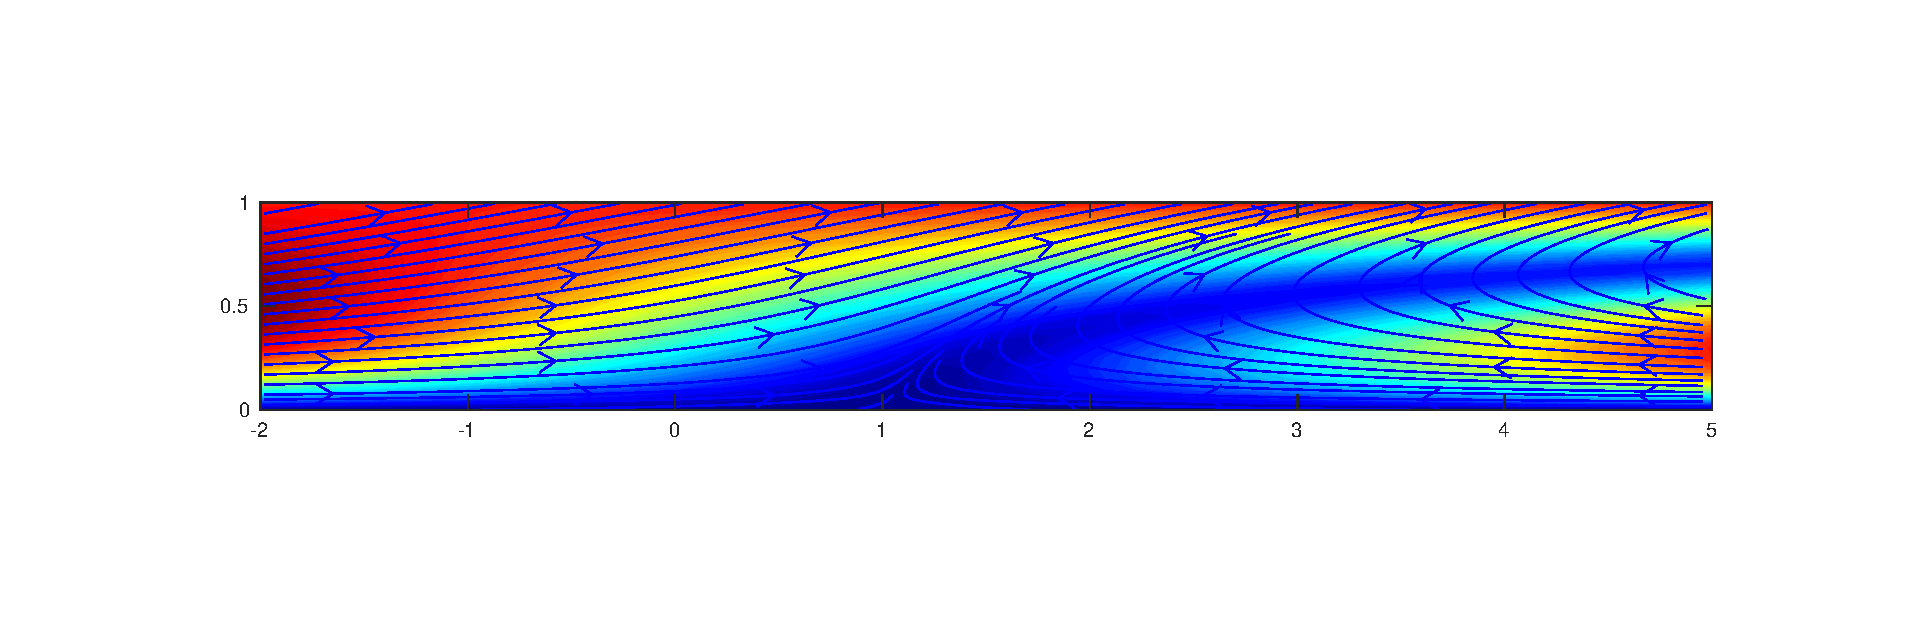
\includegraphics[width=0.90\textwidth,trim = {10mm 30mm 10mm 20mm}, clip]{./fig/Ese75contour.eps}
   \caption{Linee di corrente e modulo della velocità.}
\end{figure}

\begin{figure}[h!]
\centering
   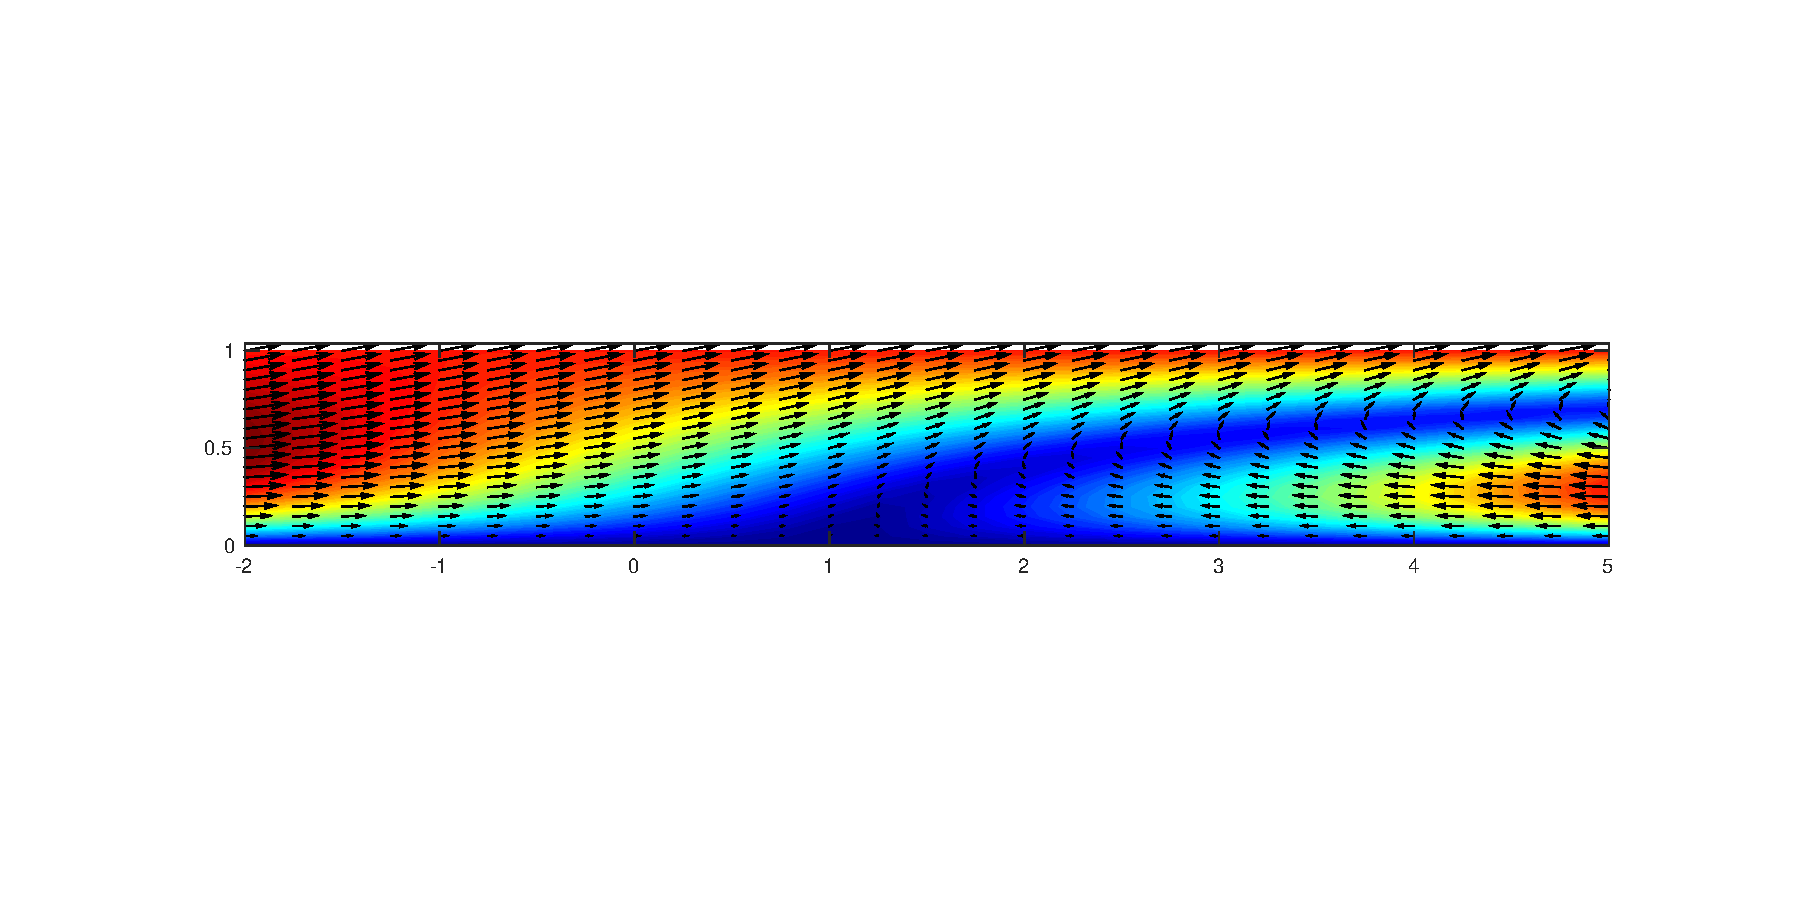
\includegraphics[width=0.90\textwidth,trim = {10mm 50mm 10mm 40mm}, clip]{./fig/Ese75quiver.eps}
   \caption{Campo di velocità e modulo della velocità.}
\end{figure}

\begin{figure}[h!]
\centering
   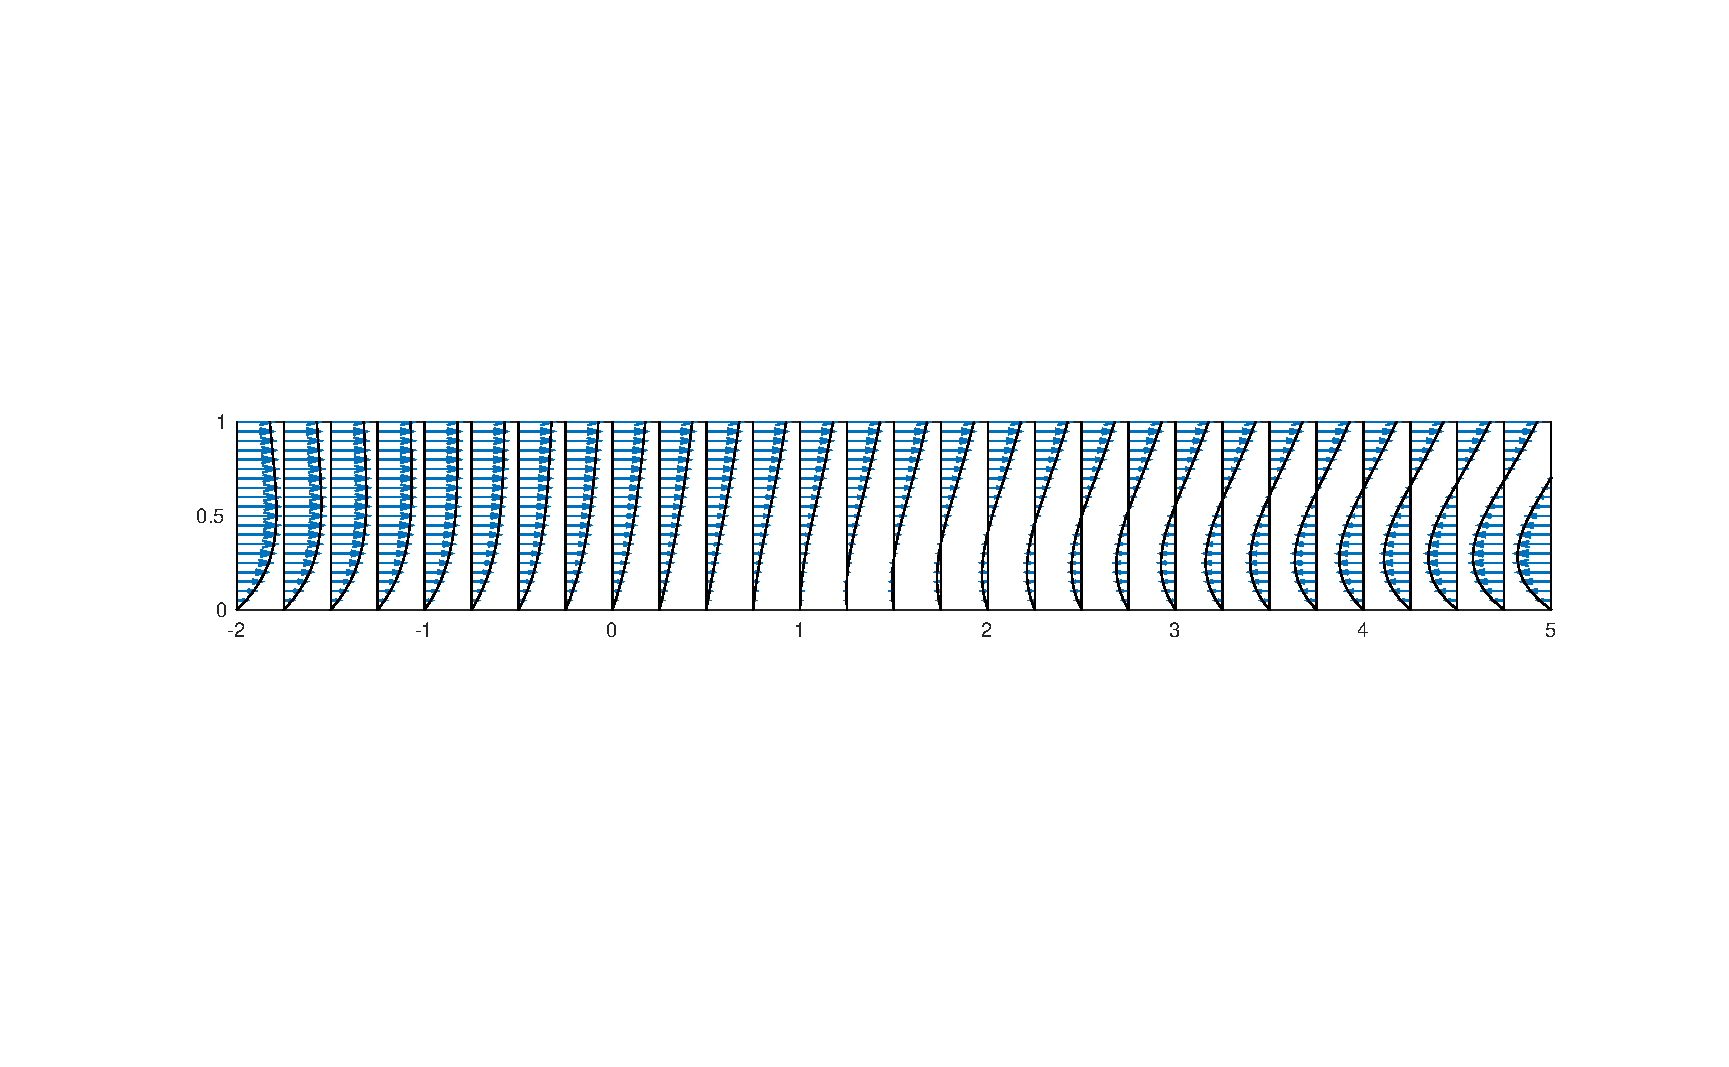
\includegraphics[width=0.90\textwidth,trim = {10mm 60mm 10mm 60mm}, clip]{./fig/Ese75u.eps}
   \caption{Andamento della componente orizzontale $u(y)$ in diverse stazioni x.}
\end{figure}

Se si ipotizza che il moto del fluido sia governato dalle equazioni di 
 Navier-Stokes per fluido incomprimibile (così facendo, si abbandonano
 le ipotesi di non viscosità del fluido e irrotazionalità della corrente, 
 proprie dell'Aerodinamica; in realtà questo è già stato fatto nel testo
 del problema, imponendo un profilo di velocità che soddisfa la condizione
 di adesione a parete...) è possibile ricostruire il campo di velocità e di 
 pressione. Utilizzando il vincolo di incomprimibilità e le condizioni
 al contorno a parete ($y=0$), si può calcolare la componente di velocità
 $v(x,y)$ perpendicolare alla parete
 \begin{equation}
  v(x,y) = - ln | 1 + y | + atan \ y
 \end{equation}
 Utilizzando le equazioni stazionarie di Navier-Stokes è possibile 
 determinare il campo di pressione $P(x,y)$. La pressione (a meno di 
 costanti di integrazione) e la derivata in direzione $x$ valutate
 a parete valgono
 \begin{equation}
 \begin{cases}
  P(x,0) & = \dfrac{1}{Re} ( 2 x^2 - 2 x ) \\
  \dfrac{\partial P}{\partial x}(x,0) & = \dfrac{1}{Re} ( 4 x - 2 )
 \end{cases}
 \end{equation}
 Si noti che nel punto di separazione $x_s=1$, la derivata $\partial P/
 \partial x (x_s,0) = 2 / Re$ è positiva (come era logico attendersi, per la
 condizione necessaria di incipiente separazione).

 
 

%\begin{figure}[h!]
%\centering
%   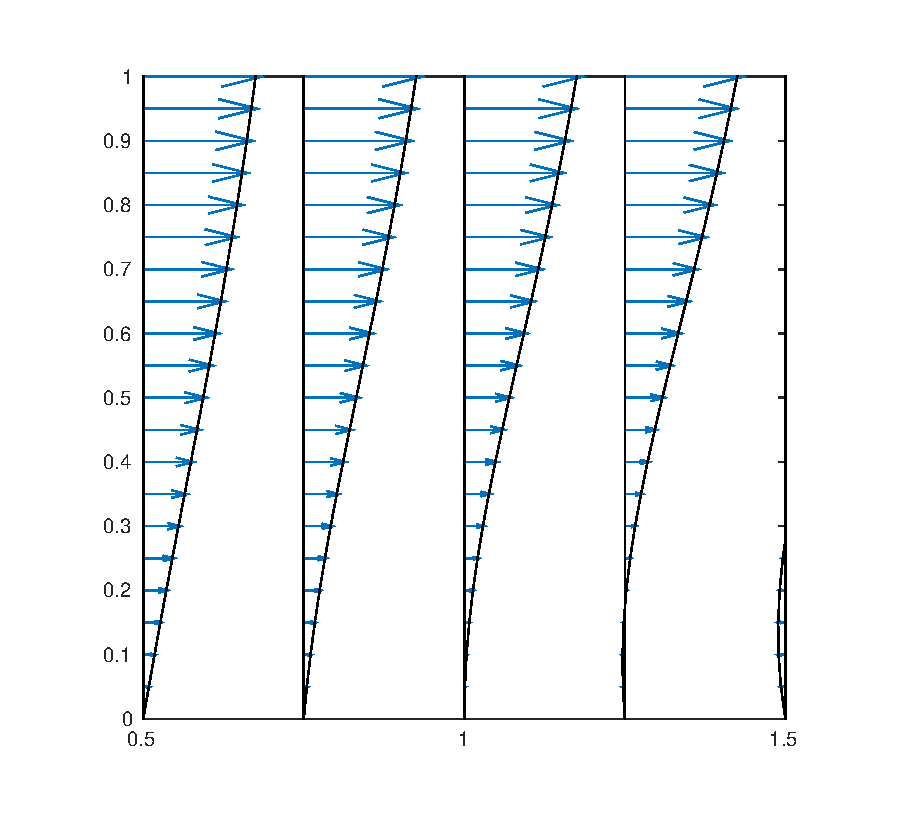
\includegraphics[width=0.90\textwidth]{./fig/Ese75uSep.eps}
%   \caption{Ingrandimento sul punto di separazione.}
%\end{figure}



\newpage
\clearpage
\noindent
\begin{tabular}{c}
\begin{minipage}[b]{0.95\textwidth}
\begin{exerciseS}[Separazione su parete piana]
Si assuma che il profilo di velocit\`{a} $u(x,y)$ dello strato limite sulla superficie di un corpo
sia approssimabile con la seguente legge
$$
 u = 1-e^{-y/\sqrt{x}},
$$
dove $u$ \`{e} la velocit\`{a} adimensionalizzata rispetto alla velocit\`{a} esterna, $x$ \`{e} la 
coordinata adimensionale di parete localmente rettilinea e $y$ la coordinata adimensionale in direzione
normale alla parete stessa. Determinare l'andamento dello spessore di spostamento $\delta$ in funzione 
della coordinata $x$ lungo la parete. Lo strato limite in questione separa? Se si per quale valore di $x$?
\vspace{0.5cm}

($\delta(x)=\sqrt{x}$, lo strato limite non separa mai se non nel limite di $x\rightarrow\infty$)
\end{exerciseS}
\end{minipage}
\end{tabular}



\sol

\partone
 Separazione. Spessori di strato limite.

\begin{equation}
  \delta(x) = \int_{0}^{\infty} \left( 1 - \frac{u(y)}{U_e} \right) dy
\end{equation}

\parttwo

\begin{itemize}
\item Spessore di spostamento. Il profilo di velocità è già adimensionalizzato sulla "velocità esterna". Utilizzando la definizione di spessore di spostamento, si ottiene:
\begin{equation}
\begin{aligned}
  \delta(x) & = \int_{0}^{\infty} \left( 1 - u(y) \right) dy = \\
  & = \int_{0}^{\infty} (1 - (1-e^{-y/\sqrt{x}}))dy  = \\
  & = \int_{0}^{\infty} e^{-y/\sqrt{x}} dy = \\
  & = -\sqrt{x} [e^{-y/\sqrt{x}}]\big|_{y=0}^{\infty}
\end{aligned}
\end{equation}

E quindi: $\delta(x) = \sqrt{x}$.



\item Separazione. La condizione di separazione è $\frac{\partial u}{\partial y}\big|_{y=0} = 0$.

\begin{equation}
\begin{aligned}
  \frac{\partial u}{\partial y}  = 
  \frac{\partial}{\partial y} \displaystyle \left[   1-e^{-y x^{-1/2}} \right] = 
   x^{-1/2} e^{-y x^{-1/2}}
\end{aligned}
\end{equation}



Si osserva che $\frac{\partial u}{\partial y}\big|_{y=0}$ non si annulla mai:
\begin{equation}
  \displaystyle\frac{\partial u}{\partial y}\displaystyle\Big|_{y=0} = \frac{1}{\sqrt{x}}
\end{equation}

\end{itemize}


\newpage
\clearpage
\noindent
\begin{tabular}{c}
\begin{minipage}[b]{0.95\textwidth}
\begin{exerciseS}[Doppietta]
Trovare il campo di moto generato da una doppietta.
Sovrapporre ad esso una corente uniforme con lìvelocità asintotica lungo x, per trovare la corrente attorno al cilindro: stabilire il legame tra l'intensità della doppietta, la velocità asintotica e il raggio del cilindro.
\end{exerciseS}
\end{minipage}
\end{tabular}


\sol

\partone
  Soluzioni elementari dell'equazione di Laplace. 
  Sovrapposizione di soluzioni elementari. Doppietta. Corrente attorno
  al cilindro.

\parttwo
  Dopo aver ricordato la definizione di doppietta, si calcolano il campo di moto e il potenziale cinetico da essa generato. Fatto questo, si sommano gli effetti della corrente indisturbata e si trovano le condizioni in cui esiste un raggio $a$ (il raggio del cilindro) per il quale si annulla la velocità normale per ogni $\theta \in [0, 2\pi]$.

\begin{itemize}
\item Definizione di doppietta ed equazioni. Per $d$ finito:

  \begin{equation}
  \begin{aligned}
    \phi & = \phi^+ + \phi^- = \\
    & = \frac{q}{2\pi}\ln{\sqrt{\displaystyle\left( x - \frac{d}{2} \right)^2 + y^2}} - 
    \frac{q}{2\pi}\ln{\sqrt{\displaystyle\left( x + \frac{d}{2} \right)^2 + y^2}} = \\
    & = \frac{q}{4\pi}\ln{\frac{( x - d/2 )^2 + y^2}{( x + d/2 )^2 + y^2}}
  \end{aligned}
  \end{equation}
Facendo tendere $ d \to 0$ in modo tale che $qd = \mu$ sia finito e diverso da zero, sfruttando $\ln(1+x)\sim x$ per $x \to 0$:
\begin{equation}
  \frac{q}{4\pi}\ln{\frac{( x - d/2 )^2 + y^2}{( x + d/2 )^2 + y^2}} = 
  \frac{q}{4\pi}\ln\displaystyle\left[1- \frac{2xd}{( x + d/2 )^2 + y^2}\right] \sim
  -\frac{qd}{2\pi}\frac{x}{(x^2 + y^2)}
\end{equation}
Quindi, il potenziale cinetico della doppietta espresso in coordinate cartesiane e cilindriche è:
\begin{equation}
  \phi = -\frac{\mu}{2\pi}\frac{x}{(x^2 + y^2)} = -\frac{\mu}{2\pi r}\cos \theta
\end{equation}
Le componenti cartesiane della velocità sono:
\begin{equation}
 \begin{cases}
  u = \frac{\partial \phi}{\partial x} = \frac{\mu}{2\pi}\frac{x^2 - y^2}{(x^2 + y^2)^2} =  \frac{\mu}{2\pi}\frac{\cos^2 \theta - \sin^2 \theta}{r^2} = \frac{\mu}{2\pi}\frac{\cos(2\theta)}{r^2} \\
  v = \frac{\partial \phi}{\partial y} = \frac{\mu}{2\pi}\frac{2xy}{(x^2 + y^2)^2} =  \frac{\mu}{2\pi}\frac{2\cos \theta \sin \theta}{r^2} = \frac{\mu}{2\pi}\frac{\sin(2\theta)}{r^2} \\
 \end{cases}
\end{equation}
Quelle cilindriche:
\begin{equation}
 \begin{cases}
  u_r = u \cos\theta + v \sin\theta = 
  \frac{\mu}{2\pi r^2}[\cos(2\theta)\cos\theta + 
  \sin(2\theta)\sin\theta ] = 
  \frac{\mu}{2\pi r^2} \cos\theta\\
  u_\theta = -u \sin\theta + v \cos\theta = 
  \frac{\mu}{2\pi r^2}[- \cos(2\theta)\sin\theta + 
  \sin(2\theta)\cos\theta] = 
  \frac{\mu}{2\pi r^2} \sin\theta\\
 \end{cases}
\end{equation}

\item
Si svovrappone alla soluzione appena trovata, quella della corrente uniforme

\begin{equation}
  \begin{cases}
    u_r = \displaystyle\left( U_\infty + \frac{\mu}{2\pi r^2} \right)\cos\theta \\
    u_\theta = \displaystyle\left( - U_\infty + \frac{\mu}{2\pi r^2} \right)\sin\theta \\
  \end{cases}
\end{equation}

\item 
Si impongono le condizioni al contorno $u_r(a,\theta) = 0, \theta \in [0, 2\pi]$, per trovare il legame
tra il raggio del cilindro $a$, la velocità asintotica $U_\infty$ e l'intensità della doppietta $\mu$.
\begin{equation}
  0 = u_r(a,\theta) =  \displaystyle\left( U_\infty + \frac{\mu}{2\pi a^2} \right)\cos\theta
  \Rightarrow \frac{\mu}{2\pi} = - a^2 U_\infty 
\end{equation}

\item
Si ricostruisce infine la soluzione (alla quale è immediato sommare un eventuale vortice nel centro del cilindro) del flusso potenziale all'esterno del cilindro:

\begin{equation}
  \begin{cases}
    u_r = U_\infty \displaystyle\left(1 - \frac{a^2}{r^2}  \right)\cos\theta \\
    u_\theta = - U_\infty \displaystyle\left(1 + \frac{a^2}{r^2}  \right)\sin\theta \\
  \end{cases}
\end{equation}
\end{itemize}


\newpage
\clearpage

\begin{exerciseS}[Metodo di Pistolesi]
Il metodo di Pistolesi è un primo metodo rudimentale per la modellazione di profili
bidimensionali nell'ambito della teoria a potenziale. Il profilo viene approssimato con una lamina piana. 
L'effetto del profilo viene modellato tramite la sovrapposizione a una corrente asintotica di un vortice posto a un quarto di corda (corrispondente all'incirca con la posizione del centro aerodinamico - def...). Il valore della circolazione (e quindi della portanza) viene ricavato imponendo le condizioni al contorno in un punto di controllo sul profilo.

Assumendo sia valida l'approssimazione per piccoli angoli $\sin \alpha \sim \alpha$, confrontando la formula della portanza $l = \frac{1}{2} \rho U^2 c c_L$ con quella ottenuta dal teorema di Kutta-Joukowski, ipotizzando un valore di $c_{L_\alpha} = 2\pi$,
si trovi il punto di controllo nel quale deve essere imposta la condizione al contorno.

Quale condizione al contorno va imposta e perchè?
\end{exerciseS}


\sol

\partone Metodi a pannelli. Metodo di Pistolesi. Aerodinamica potenziale.
  
\parttwo
La condizione da imporre è quella di tangenza: la velocità nel punto di controllo deve essere tangente alla lamina piana.

Definita $b$ la distanza del punto di controllo dal centro aerodinamico, si impone la condizione al contorno in tale punto: deve essere nulla la componente normale alla lamina della velocità ottenuta come sovrapposizione della corrente asintotica e della corrente indotta dal vortice.

\begin{equation}
  0 = \frac{\Gamma}{2\pi b} + U_\infty \sin \alpha \qquad \Rightarrow \qquad 
  \Gamma = - 2\pi b U_\infty \alpha
\end{equation}

Inserita nel teorema di Kutta-Joukowski  $l = -\rho \Gamma U_\infty = \rho U_\infty^2 b 2\pi \alpha$ e confrontata alla formula della portanza $l = \frac{1}{2} \rho U^2 c c_L$, si ottiene

\begin{equation}
  b = \frac{c}{2}
\end{equation}

Quindi nel metodo di Pistolesi, il centro aerodinamico è posizionato $\frac{1}{4}$  di corda, mentre il punto di controllo è posizionato a $\frac{3}{4}$ di corda.

\vspace{0.5cm}
\textit{Osservazioni.} 
\begin{itemize}

\item \'E possibile simulare l'interazione tra più profili. Con metodi a pannelli un po' più raffinati
   (Hess Smith, Morino,...) è possibile simulare l'interazione tra corpi aerodinamici di forma qualsiasi,
   ricordandosi che le informazioni ottenute sono valide sotto le ipotesi dell'aerodinamica a potenziale:
   non devono verificarsi grandi separazioni, la vorticità deve essere confinata in una regione sottile
   (numero di Reynolds elevato).
  

\item Quale può essere un metodo per simulare l'effetto di una superficie piana infinita (effetto suolo)?

\end{itemize}

\newpage
\clearpage

\begin{exerciseS}[Effetto suolo e interazione profili]
Usare il metodo di Pistolesi per ottenere delle informazioni qualitative sul coefficiente
 di portanza
\begin{itemize}
 \item di un profilo in effetto suolo 
 \item di due profili, in funzione della posizione reciproca
\end{itemize}
\end{exerciseS}

\paragraph{Confronto con i risultati ottenuti con il metodo di Hess Smith:
 effetto suolo.}
Con il metodo delle immagini è possibile calcolare l'effetto che ha la
 presenza di una parete orizzontale (parallela alla velocità asintotica)
 sul coefficiente di portanza di un profilo NACA2412 con incidenza 
 $\theta = 2\degree$. Il coefficiente di portanza in ``aria libera'' è
 $c_{L0} = 0.481$. La distanza del profilo dalla parete è adimensionalizzata
 sulla corda.

\begin{tabular}{cc}
\begin{minipage}{0.47\textwidth}
\begin{verbatim}
  h/c      cL     DcL/cL0
-----------------------------
 0.500   0.680     0.261
 1.000   0.536     0.112
 1.500   0.508     0.054
 2.000   0.498     0.033
 2.500   0.493     0.022
 3.000   0.490     0.016
 3.500   0.488     0.012
\end{verbatim}
\end{minipage}
&
\begin{minipage}{0.47\textwidth}
\begin{center}
\begin{tikzpicture}
\begin{axis}[axis x line=bottom, axis y line=middle, domain=-1.2:3.2, xlabel={$c_L/c_{L0}$}, ylabel={$h/c$},xmin=1.0,xmax=1.5,ymin=0.0,ymax=3.5]
\addplot coordinates{
(  1.261 ,  0.500  ) 
(  1.112 ,  1.000  ) 
(  1.054 ,  1.500  ) 
(  1.033 ,  2.000  ) 
(  1.022 ,  2.500  ) 
(  1.016 ,  3.000  ) 
(  1.012 ,  3.500  ) 
};
\legend{$c_L/c_{L0}$}
\end{axis}
\end{tikzpicture}
\end{center}
\end{minipage}
\end{tabular}

\paragraph{Confronto con i risultati ottenuti con il metodo di Hess Smith:
 due profili.} Quando due profili sono investiti da una corrente, ognuno
 di essi influenza l'altro. Come primo esempio vengono usati due profili
 NACA0012, con la stessa corda. Il secondo profilo viene messo in scia al
 primo a distanza di 3 corde. La prima prova consiste nel mantenere il 
 secondo profilo a incidenza nulla rispetto alla velocità asintotica, 
 aumentando l'incidenza del primo. Il primo profilo genera una portanza
 inferiore a un profilo in aria libera, mentre il secondo è deportante: il
 primo profilo induce una velocità verso il basso sul profilo in coda, che
 quindi vede un'incidenza non nulla, ma negativa.
\begin{center}
\begin{verbatim}
 theta2 = 0.0\degree
-------------------------------
 theta1    cL1     cL2    cL10 
-------------------------------
   2.5°  0.286  -0.045   0.297 
   5.0°  0.571  -0.089   0.594 
\end{verbatim}
\end{center}

 La seconda prova consiste nel mantenere il primo profilo a incidenza nulla
 rispetto alla velocità asintotica e aumentare l'incidenza del profilo in scia.
 Il secondo profilo ha un coefficiente di portanza minore rispetto a quello
 di un profilo in aria libera; il primo profilo è anch'esso portante: il
 profilo in scia induce una velocità verso l'alto sul primo profilo che quindi
 vede un'indicenza positiva.
\begin{center}
\begin{verbatim}
 theta1 = 0.0°
-------------------------------
 theta2    cL1     cL2    cL20 
-------------------------------
   2.5°  0.064   0.287   0.297 
   5.0°  0.128   0.573   0.594 
\end{verbatim}
\end{center}
 La portanza risultante è maggiore a quella che si otterrebbe considerando
 la somma della portanza generata singolarmente dai due profili. Per esempio,
 per $\theta = 2.5°$:
\begin{equation}
\begin{aligned}
 c_{L1} + c_{L2} & > c_{L01} + c_{L02} \\
  0.064 + 0.287  & >  0.000  +  0.297  \\
          0.351  & >  0.297
\end{aligned}
\end{equation}
Lo stesso effetto viene osservato con due profili più vicini tra loro. La corda
 del profilo secondario è la metà di quella del profilo principale.
 Il profilo principale ha incidenza $\theta_1 = -0.5°$ rispetto alla velocità
 asintotica, quello secondario $\theta_2 = 12°$. La presenza del secondo 
 profilo fa aumentare significativamente la portanza del profilo principale.

\begin{tabular}{ll}
\begin{minipage}{0.43\textwidth}
\begin{center}
\begin{verbatim}
          +------------------------
          | theta  |   cL  |  cL0 
----------+--------+-------+-------
airfoil 1 |  -0.5° | 1.099 | 0.184
airfoil 2 |  12.0° | 0.975 | 1.656
----------+--------+-------+-------
\end{verbatim}
\end{center}
La colonna $\mathtt{cL}$ contiene i coefficienti di portanza dei profili
 disposti
 come in figura. La colonna $\mathtt{cL0}$ contiene i coefficienti di portanza
 dei
 profili presi singolarmente, senza influenza reciproca, alla stessa incidenza.
%  Per ottenere la portanza complessiva, bisogna ricordarsi che i coefficienti
%  dei due profili sono adimensionalizzati sulle rispettive corde.
 
%  -----------------------
%    cL20  theta2    cL2  
%  -----------------------
%    1.656  12.0°   0.975 
\end{minipage}
&
\begin{minipage}{0.57\textwidth}
\begin{center}
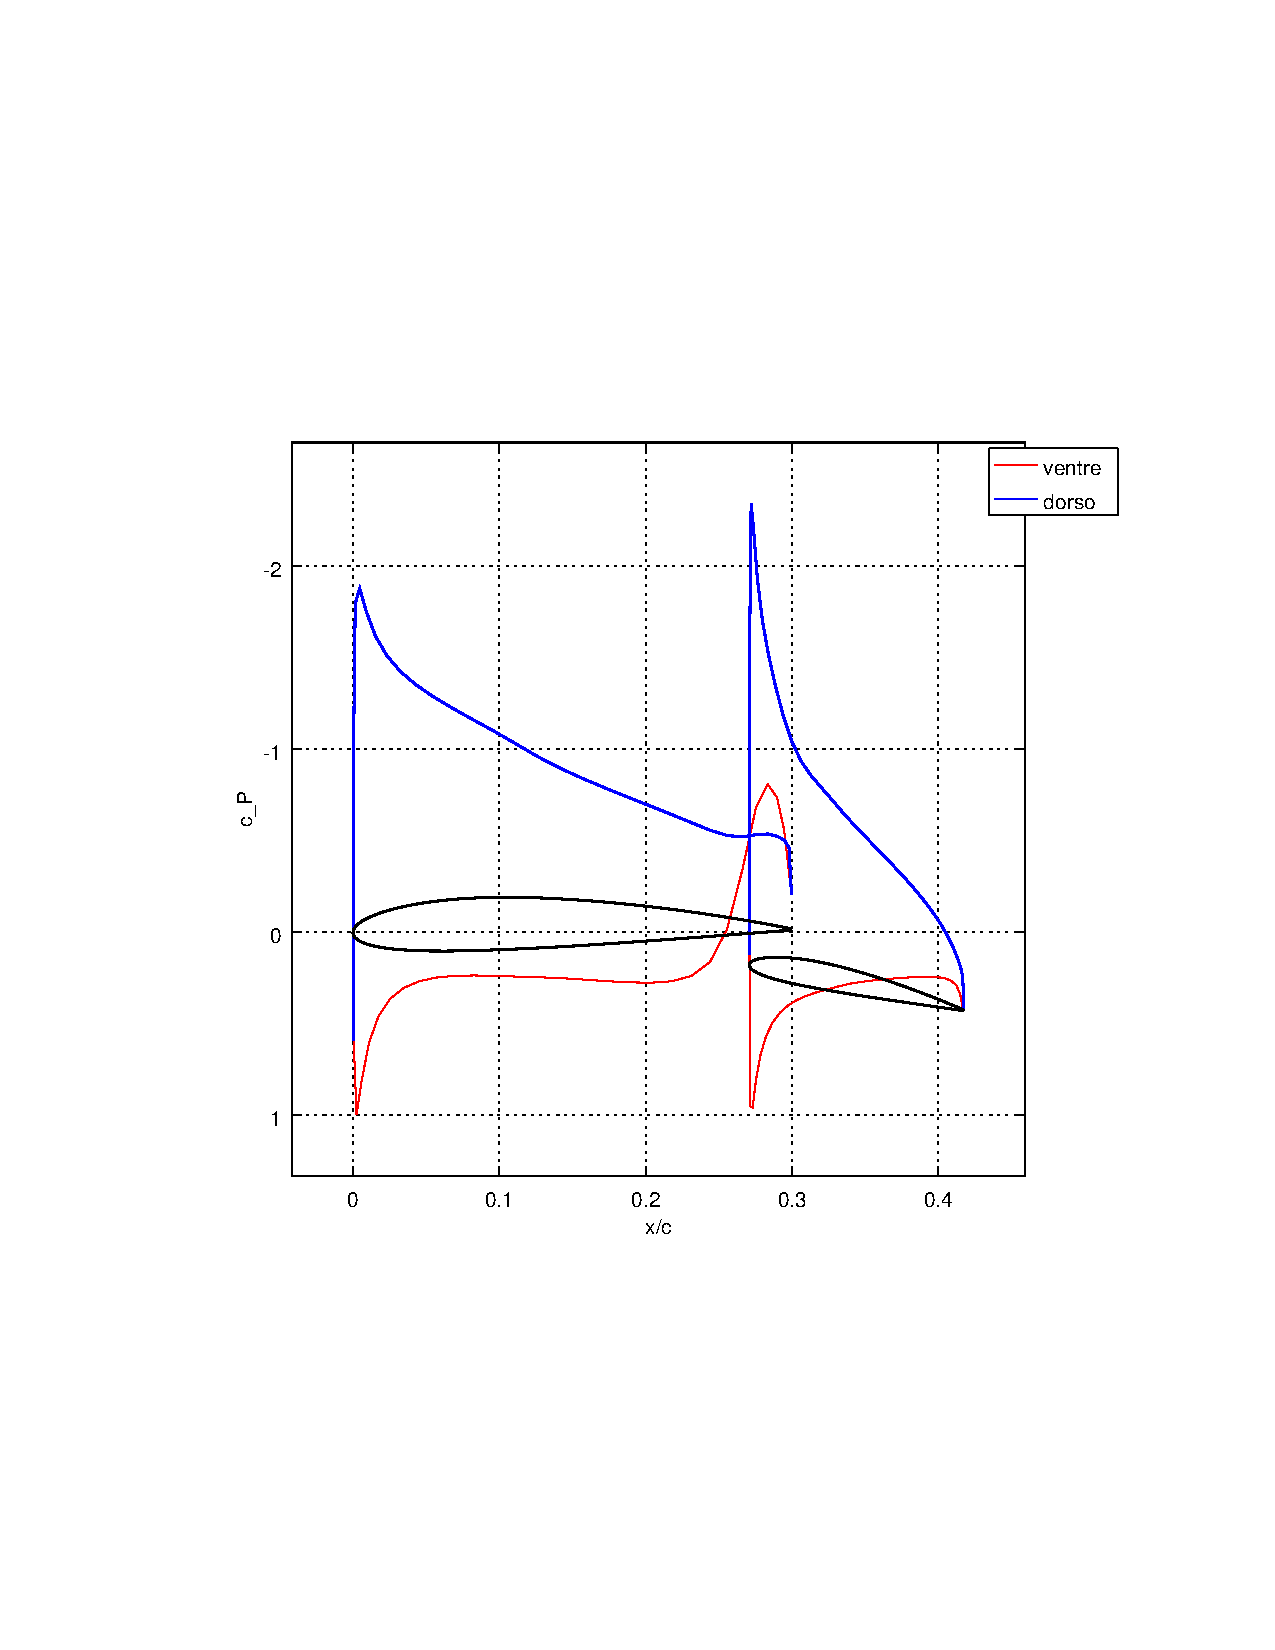
\includegraphics[width=0.95\textwidth,trim={3cm 6cm 2cm 6cm},clip]
        {./fig/Aileron.pdf}
\end{center}
\end{minipage}
\end{tabular}

Come ultimo esempio si considerano due profili NACA0012 uguali sovrapposti,
 con angolo di incidenza $\theta=5.0°$, separati da una distanza
 adimensionalizzata $y/c$ compresa tra 1 e 15. Il coefficiente di portanza
 del singolo profilo è $c_L = 0.594$.

\begin{center}
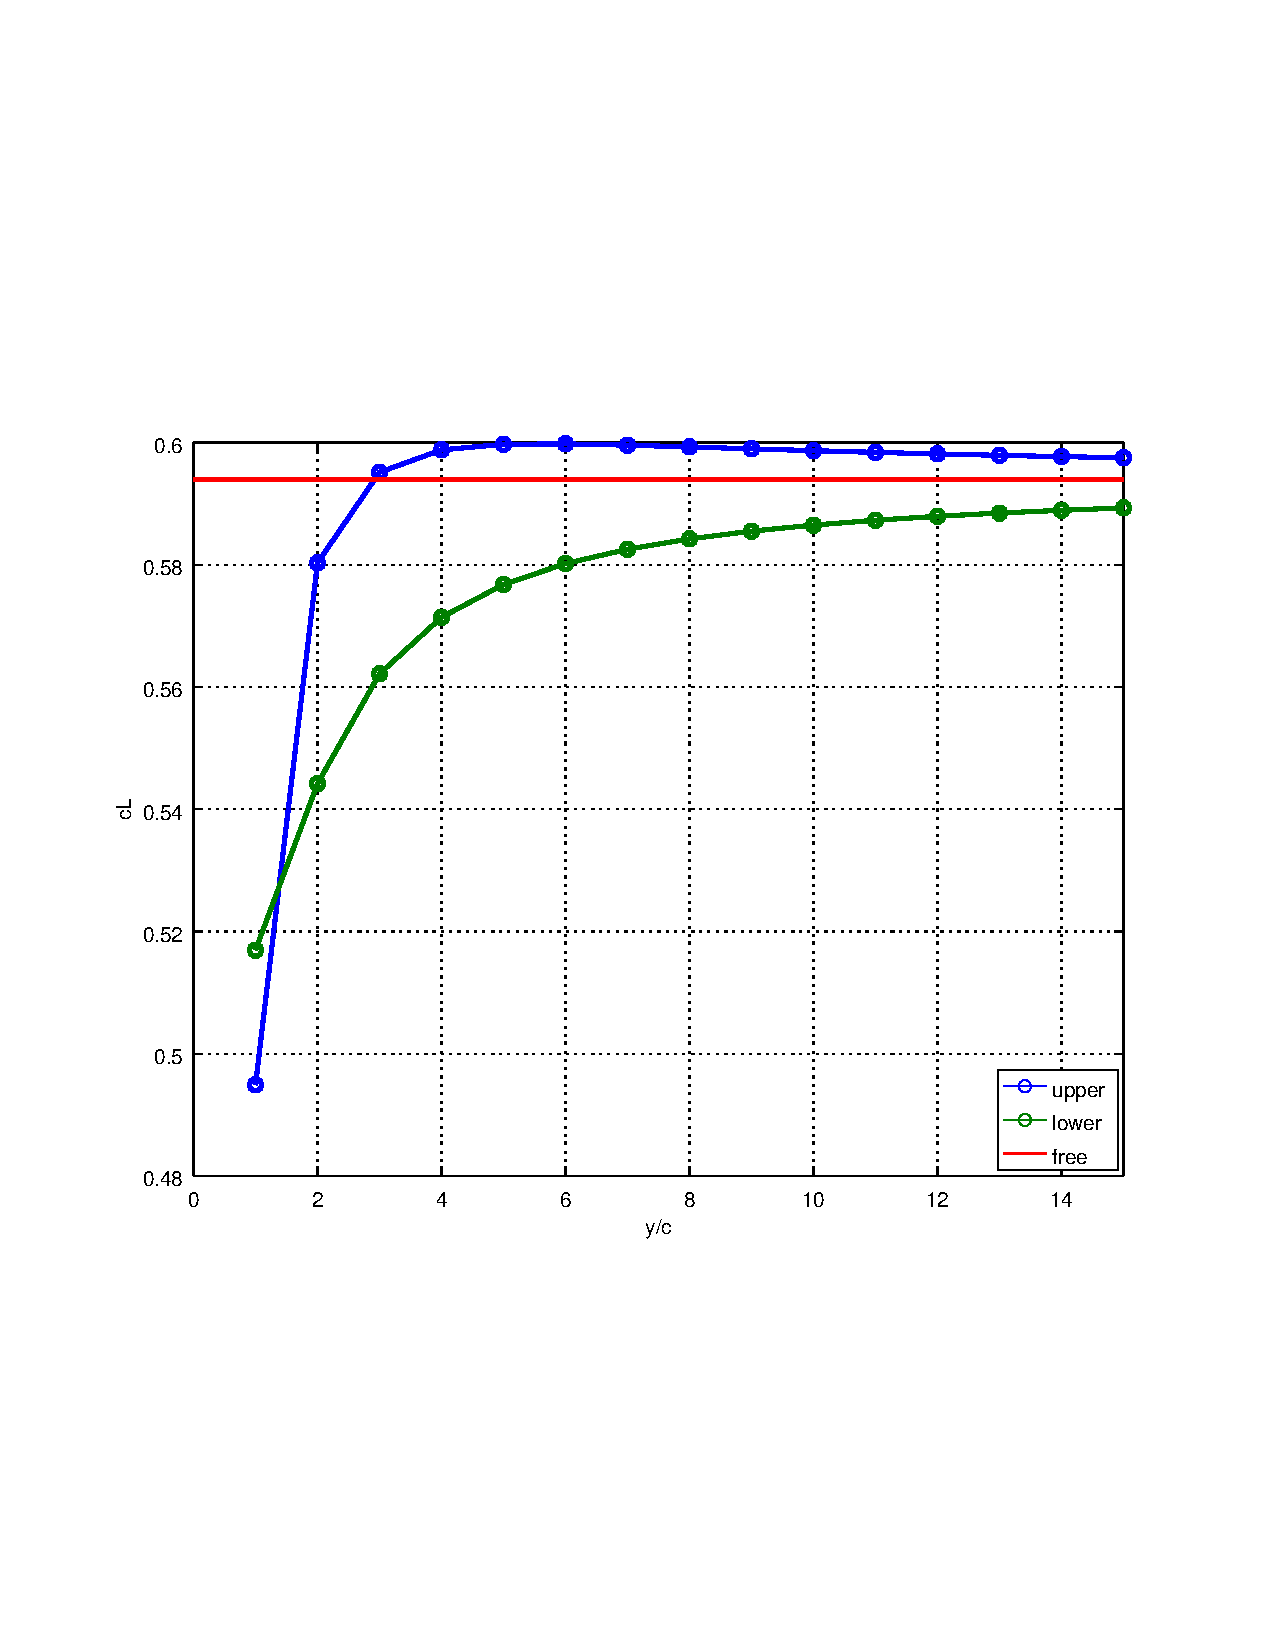
\includegraphics[width=0.60\textwidth,trim={0 5cm 0 5cm},clip]
       {./fig/vanes.pdf}
\end{center}

\noindent
Esistono alcuni esempi "esotici": ekranoplano sovietico...; esempi meno esotici:...


%%%%%%%%%%%%%%%%%%%%%%%%%%%%%%%%%%%%%%%%%%%%%%%%%%%%%%%%%%%%%%%%%%

%%%%%%%%%%%%%%%%%%%%%%%%%%%%%%%%%%%%%%%%%%%%%%%%%%%%%%%%%%%%%%%%%%

%%%%%%%%%%%%%%%%%%%%%%%%%%%%%%%%%%%%%%%%%%%%%%%%%%%%%%%%%%%%%%%%%%

%%%%%%%%%%%%%%%%%%%%%%%%%%%%%%%%%%%%%%%%%%%%%%%%%%%%%%%%%%%%%%%%%%

%%%%%%%%%%%%%%%%%%%%%%%%%%%%%%%%%%%%%%%%%%%%%%%%%%%%%%%%%%%%%%%%%%
%%%%%%%%%%%%%%%%%%%%%%%%%%%%%%%%%%%%%%%%%%%%%%%%%%%%%%%%%%%%%%%%%%

\end{document}

